%!TEX program = xelatex
\documentclass[aspectratio=43,UTF8,10pt]{ctexbeamer}

    \mode<presentation> {
    \usetheme{Madrid}
    %\setbeamertemplate{footline} % To remove the footer line in all slides uncomment this line
    \setbeamertemplate{footline}[frame number] % To replace the footer line in all slides with a simple slide count uncomment this line
    \setbeamercolor{page number in head/foot}{fg=blue}
    \setbeamertemplate{navigation symbols}{} % To remove the navigation symbols from the bottom of all slides uncomment this line
    }
    \usepackage{indentfirst}
    \setlength{\parindent}{2em}
    \usepackage{listings}
    \lstset{language=C++, showstringspaces=false, basicstyle=\small}
    \usepackage{wrapfig}
    \usepackage{graphicx}
    % \usepackage{fboxrule}
\definecolor{hanblue}{rgb}{0.27, 0.42, 0.81}
\definecolor{indiagreen}{rgb}{0.07, 0.53, 0.03}
\definecolor{indianred}{rgb}{0.8, 0.36, 0.36}
\definecolor{indianyellow}{rgb}{0.89, 0.66, 0.34}
\definecolor{babypink}{rgb}{0.96, 0.76, 0.76}
\definecolor{ao(english)}{rgb}{0.0, 0.5, 0.0}

    \definecolor{azure(colorwheel)}{rgb}{0.0, 0.5, 1.0}
    \definecolor{alizarin}{rgb}{0.82, 0.1, 0.26}
    % User Defined Block %%%%%%%%%%%%%%%%%%%%%%%%%%%%%%%%%%%%%%%%%%%%%%%%%%%%%%%%




    \newenvironment<>{blueblock}[1]{%
      \setbeamercolor{block title}{fg=white,bg=hanblue}%
    %   \setbeamercolor{block body}{fg=white,bg=bondiblue}%
      \begin{block}#2{#1}}{\end{block}}

    \newenvironment<>{greenblock}[1]{%
    % \setbeamercolor{block title}{fg=white,bg=bondiblue}%
      \setbeamercolor{block title}{fg=white,bg=indiagreen}%
    \begin{block}#2{#1}}{\end{block}}

    \newenvironment<>{redblock}[1]{%
      \setbeamercolor{block title}{fg=white,bg=indianred}%
    %   \setbeamercolor{block body}{fg=white,bg=bondiblue}%
      \begin{block}#2{#1}}{\end{block}}

    \newenvironment<>{yellowblock}[1]{%
      \setbeamercolor{block title}{fg=white,bg=indianyellow}%
      \begin{block}#2{#1}}{\end{block}}

    \lstset{language=C++,
    columns=flexible,
    basicstyle=\footnotesize\ttfamily,                                    % 设定代码字体、大小
    %numbers=left,xleftmargin=2em,framexleftmargin=2em,                   % 在左侧显示行号
    %numberstyle=\color{darkgray},                                        % 设定行号格式
    keywordstyle=\color{blue},                                            % 设定关键字格式
    commentstyle=\color{ao(english)},                                     % 设置代码注释的格式
    stringstyle=\color{brown},                                            % 设置字符串格式
    showstringspaces=false,                                              % 控制是否显示空格
    %frame=single,                                                         % 控制外框
    breaklines,                                                           % 控制是否折行
    % postbreak=\space,                                                     % 控制折行后显示的标识字符
    breakindent=5pt,                                                      % 控制折行后缩进数量
    emph={size\_t,array,deque,list,map,queue,set,stack,vector,string,pair,tuple,ostream,istream}, % 非内置类型
    emphstyle={\color{teal}},
    escapeinside={(*@}{@*)},
}

\usepackage{multicol}

%----------------------------------------------------------------------------------------
%	TITLE PAGE
%----------------------------------------------------------------------------------------



\title[\textit{C++程序设计:第六章}]{第六章~类} % The short title appears at the bottom of every slide, the full title is only on the title page

%\author[李长河]{李长河} % Your name
%\institute[CUG] % Your institution as it will appear on the bottom of every slide, may be shorthand to save space
%{
%中国地质大学(武汉)\\ % Your institution for the title page
%\medskip
%\textit{lichanghe@cug.edu.cn} % Your email address
%}
\date{} % Date, can be changed to a custom date

\begin{document}

%----------------------------------------------------------------------------------------
%	TIKZ FLOWCHART
%----------------------------------------------------------------------------------------
%\tikzstyle{startstop} = [rectangle, rounded corners, minimum width=2cm, minimum height=0.5cm, text centered, draw=black, fill=red!30, font=\tiny]
%\tikzstyle{io} = [trapezium, trapezium left angle=70, trapezium right angle=110, minimum width=0cm, minimum height=0cm, text centered, draw=black, fill=blue!30, font=\tiny]
%\tikzstyle{process} = [rectangle, minimum width=2.5cm, minimum height=1.5cm, text centered, draw=black, fill=orange!30, font=\tiny, text width=2cm]
%\tikzstyle{decision} = [diamond, minimum width=2.5cm, minimum height=2cm, text centered, draw=black, fill=green!30, font=\tiny, text width=1.8cm, aspect=1.1]

\begin{frame}
\titlepage % Print the title page as the first slide
\end{frame}


\begin{frame}{目录}
\begin{multicols}{2}
  \tableofcontents
\end{multicols}
%\tableofcontents
\end{frame}

%----------------------------------------------------------------------------------------
%	PRESENTATION SLIDES
%----------------------------------------------------------------------------------------

%--------------------

\begin{frame}[fragile]{~} % Table of contents slide, comment this block out to remove it

\begin{block}{学习目标}
\begin{enumerate}
\item 理解类的概念和基本设计原则;
\item 理解构造函数和析构函数的作用与执行过程;
\item 掌握常见运算符重载技术和静态成员的使用方法;
\item 能够运用面向对象程序设计方法设计和实现简单类;
\end{enumerate}
\end{block}

%% ------功能模块说明,请注释掉-------
%\begin{columns}[t]
%\column{0.18\textwidth}
%\begin{block}{概念}
%\end{block}
%\column{0.18\textwidth}
%\begin{blueblock}{代码}
%\end{blueblock}
%\column{0.18\textwidth}
%\begin{yellowblock}{说明}
%\end{yellowblock}
%\column{0.18\textwidth}
%\begin{greenblock}{问题/答案}
%\end{greenblock}
%\column{0.18\textwidth}
%\begin{redblock}{注意}
%\end{redblock}
%\end{columns}
%% ------功能模块说明,请注释掉-------
%
\end{frame}

%--------------------


%#####################################
\section{类的定义}
\begin{frame}[fragile]
    {6.1 类的定义}
\begin{block}{类}
类是对一个事物的\alert{属性}和\alert{操作}的描述。
\begin{itemize}
  \item 用户自定义类型;
  \item 基本思想是\alert{抽象}~\text{(abstract\index{A!abstract})}和\alert{封装}(encapsulation\index{E!encapsulation});
  \item 面向对象程序设计(object-oriented programming\index{O!object-oriented programming!object},OOP)的基础。
\end{itemize}
\end{block}

\begin{block}<2->{类的要素}
\begin{itemize}
  \item 抽象:数据(属性)抽象和函数(操作)抽象;
  \item 封装:将数据和操作结合在一起。
\end{itemize}
\end{block}
\end{frame}

\subsection{定义一个类}\label{chap6-1-1}


\begin{frame}[fragile]
    {6.1.1 定义一个类}
     \vspace{-0.5em}
\begin{greenblock}{设计分数类}
设计一个分数类:基本属性有分子和分母,操作包括约分、计算分数值等操作。
\end{greenblock}
\begin{columns}
\column{0.6\textwidth}
 \vspace{-1em}
\begin{blueblock}<2->{分数类}
 \vspace{-0.1em}\begin{lstlisting}
class Fraction {
    //数据成员,访问控制属性默认是私有
    int m_numerator = 0;  // 分子默认为0; C++11
    int m_denominator = 1;  //分母默认为1;
public://公有成员函数
    int numerator() const { return m_numerator; }
    int denominator() const { return m_denominator; }
    double value() const;  //计算分数值
    void reduce();  //约分
private:
    int gcd(int x, int y);  //求分子分母最大公约数
};
//辅助函数
void makeCommon(Fraction &a, Fraction &b);
ostream& print(ostream &out, const Fraction &f);
\end{lstlisting}%\vspace{-1.5mm}
\end{blueblock}
\column{0.35\textwidth}
\begin{block}<3->{类的语法}
\begin{itemize}
  \item 类名紧随~\textcolor{blue}{class}~关键字;
  \item 数据成员和成员函数放到一对\alert{花括号}里面;
  \item \alert{分号}结尾。
\end{itemize}
\end{block}
\begin{redblock}<4->{建议:成员命名}
\begin{itemize}
  \item 一个类的数据成员名通常以~m\_~开头;
  \item 成员函数名尽量使用动词短语,如~reverse。
\end{itemize}
\end{redblock}
\end{columns}
\end{frame}

%#####################################
\subsection{定义和使用成员函数}
%--------------------
\begin{frame}[fragile]
    {6.1.2 定义和使用成员函数}
\begin{block}{定义成员函数}
\begin{itemize}
  \item 成员函数的声明必须放到类的内部
  \item 成员函数的定义
  \begin{itemize}
    \item 类的内部:建议为\alert{内联函数};
    \item 类的外部: 可利用~\textcolor{blue}{inline}~指明其为内联函数。
  \end{itemize}
  \item 类外定义需要使用\alert{作用域符}标明成员函数所属的类;
\end{itemize}
\end{block}
\begin{blueblock}<2->{类外定义成员函数}
 \vspace{-0.1em}\begin{lstlisting}
inline double Fraction::value() const{
    return static_cast<double>(m_numerator) / m_denominator;
}
void Fraction::reduce(){
    int n=gcd(m_numerator, m_denominator); //获取分子分母的最大公约数
    m_denominator /= n;
    m_numerator /= n;
}
\end{lstlisting}
\end{blueblock}

\end{frame}


%--------------------
\begin{frame}[fragile]
    {6.1.2 定义和使用成员函数\normalsize{~---~this~指针}}

\begin{blueblock}<1->{使用~value~成员函数}
 \vspace{-2.5mm}\begin{lstlisting}
Fraction a, *p = &a;
cout << a.value() <<" "<< p->value() << endl; //打印默认值0
\end{lstlisting}\vspace{-1.5mm}
\onslide<2-> a的数据成员如何传到value成员函数中?
\end{blueblock}

\begin{blueblock}<3->{编译器转化~value~成员函数声明}
 \vspace{-2.5mm}\begin{lstlisting}
double value(Fraction *const this) const;//伪代码,说明成员函数的执行过程
\end{lstlisting}\vspace{-1.5mm}
\end{blueblock}

\begin{blueblock}<3->{~value~成员函数等价调用}
 \vspace{-2.5mm}\begin{lstlisting}
a.value(&a);
\end{lstlisting}\vspace{-1.5mm}
\end{blueblock}

\begin{block}<4->{this~指针}
\begin{itemize}
  \item 指向调用成员函数对象的\alert{const指针(指针常量)},运行代码演示
\end{itemize}
 \vspace{-0.5em}\begin{lstlisting}
double Fraction::value() const{
    return static_cast<double>(this->m_numerator) / this->m_denominator;
}
\end{lstlisting}
\end{block}
\end{frame}



%--------------------
\begin{frame}[fragile]
    {6.1.2 定义和使用成员函数\small{~---~const~成员函数}}

\begin{block}<1->{常量成员函数(const member function\index{C!const!const member function})}
\begin{itemize}
  \item 函数参数列表后面(圆括号后面)引入~\textcolor{blue}{const}~关键字;
  \item this指针指向const对象;
  \item 禁止在函数体内部对数据成员进行写操作。
\end{itemize}

\end{block}
\begin{blueblock}<2->{示例}
 \vspace{-2.5mm}\begin{lstlisting}
double value() const;
\end{lstlisting}\vspace{-1.5mm}
\end{blueblock}
\begin{blueblock}<3->{等价于}
 \vspace{-2.5mm}\begin{lstlisting}
double value(const Fraction *const this);
\end{lstlisting}\vspace{-1.5mm}
this~指针是一个指向~\textcolor{blue}{const}~对象的~\textcolor{blue}{const}~指针。
\end{blueblock}
\end{frame}




%#####################################
\subsection{定义辅助函数}
%--------------------
\begin{frame}[fragile]
    {6.1.3 定义辅助函数}

\begin{block}<1->{辅助函数}
一个类需要一些普通函数来辅助完成某些操作,不是类的成员函数,从概念上属于类的接口。
\begin{itemize}
  \item 通常将它们的声明和类的定义放到同一个头文件内;
  \item 定义和类成员函数的定义放到同一个源文件内。
\end{itemize}
\end{block}
\begin{blueblock}<2->{示例}
 \vspace{-2.5mm}\begin{lstlisting}
ostream& print(ostream &out, const Fraction &f) {
    out << f.numerator() << "/" << f.denominator();
    return out;
}
Fraction a;
print(cout,a);//打印0/1
\end{lstlisting}\vspace{-1.5mm}
\end{blueblock}
\end{frame}


\subsection{访问控制}\label{chap6-1-4}
%--------------------
\begin{frame}[fragile]
    {6.1.4 访问控制}

\begin{block}<1->{封装的意义}
\begin{itemize}
  \item 类的开发者:有利于程序的模块化设计,提高代码的重用性;
  \item 类的使用者:隐藏类的实现细节,使用者不能在类的外面操控数据成员,形成一种保护机制。
\end{itemize}
\end{block}

\begin{block}<2->{访问控制}
\begin{itemize}
  \item<2-> 如何实现访问控制?
  \item<3-> \alert{访问限定符}(access specifiers\index{A!access specifiers}):控制成员对外的可见性。
\end{itemize}
\end{block}

\begin{block}<4->{访问限定符}
\begin{itemize}
  \item \textcolor{blue}{public}~:成员对外是公开的,可以在程序的任何地方访问;
  \item \textcolor{blue}{private}~:成员不对外公开,只在类的内部使用(成员函数内)。
\end{itemize}
\end{block}

\end{frame}

\begin{frame}[fragile]
    {6.1.4 访问控制}

\begin{greenblock}{下面函数是否正确?}
 \vspace{-2.5mm}\begin{lstlisting}
ostream& print(ostream &out, const Fraction &f) {
    out << f.m_numerator << "/" << f.m_denominator; //错误:无法访问私有成员
    return out;
}
\end{lstlisting}\vspace{-1.5mm}
  \onslide<2-> 利用~\textcolor{blue}{class}~定义的类,如果没有显式指明成员的访问属性,则默认为~\textcolor{blue}{private}。
\end{greenblock}

\begin{redblock}<3->{私有成员函数:对外是隐藏的,只能在类内部的成员函数中使用}
 \vspace{-2.5mm}\begin{lstlisting}
private:
    int gcd(int x, int y);
\end{lstlisting}\vspace{-1.5mm}
\begin{lstlisting}
void Fraction::reduce(){
    int n=gcd(m_numerator, m_denominator); //获取分子分母的最大公约数
    m_denominator /= n;    m_numerator /= n;
}
\end{lstlisting}
 \vspace{-0.1em}
\end{redblock}

\begin{redblock}<4->{\textcolor{blue}{class}~和~\textcolor{blue}{struct}}
\begin{itemize}
  \item 使用~\textcolor{blue}{class}~定义的类中成员的访问属性默认为~\textcolor{blue}{private};
  \item 使用~\textcolor{blue}{struct}~定义的类中成员的访问属性默认为~\textcolor{blue}{public};
\end{itemize}
\end{redblock}


\end{frame}


\subsection{友元}\label{chap6-1-5}
\begin{frame}[fragile]
    {6.1.5 类的定义\small{~---~友元函数}}

\begin{block}<1->{友元函数}
类的辅助函数,声明为类的友元之后,它们就可以访问类的非公有成员。
\begin{itemize}
  \item 辅助函数的声明必须放到类的内部;
  \item 使用关键字~\textcolor{blue}{friend}~进行说明;
  \item 非类成员函数,仅显示授予访问权限。
\end{itemize}
\end{block}


\end{frame}


\begin{frame}[fragile]
    {6.1.5 类的定义\small{~---~友元函数}}
\begin{block}<1->{友元函数的声明}
 \vspace{-2.5mm}\begin{lstlisting}
class Fraction {
    //类的辅助函数声明为友元;
    friend ostream& print(ostream &out, const Fraction &f);
    friend void makeCommon(Fraction &a, Fraction &b);
    //其它成员与之前一致
};
//Fraction类辅助函数声明
void makeCommon(Fraction &a, Fraction &b);
ostream& print(ostream &out, const Fraction &f);
\end{lstlisting}\vspace{-1.5mm}
\end{block}

\begin{block}<2->{友元函数的定义}
 \vspace{-2.5mm}\begin{lstlisting}
ostream& print(ostream &out, const Fraction &f) {
    out << f.m_numerator << "/" << f.m_denominator;//正确:可以访问私有成员
    return out;
}
\end{lstlisting}\vspace{-1.5mm}
\end{block}
\end{frame}


\begin{frame}[fragile]
    {6.1.5 类的定义\small{~---~友元类}}
\begin{block}<1->{友元类}
将其它类或其它类的成员函数声明为该类的友元。
\end{block}

\begin{greenblock}<2->{问题}
下面定义两个类:Point~类和~Circle~类,并将~Circle~类声明为~Point~ 类的友元,使~Circle~类的成员函数可以直接访问~Point~类的私有成员。
\end{greenblock}

\end{frame}


\begin{frame}[fragile]
    {6.1.5 友元\small{~---~友元类}}
\begin{block}{友元类的定义}
 \vspace{-2.5mm}\begin{lstlisting}
class Circle; //前向声明
class Point {
    friend class Circle;
private:
    double m_x = 0, m_y = 0;//x和y坐标
};
class Circle {
    Point m_center; //圆心
    double m_radius = 1.0;//半径
public:
    void moveXTo(double val) {//将圆心沿x轴移动到指定位置
       m_center.m_x = val;//直接访问Point私有成员m_x
    }
};
\end{lstlisting}\vspace{-1.5mm}
\end{block}
\end{frame}

\begin{frame}[fragile]
    {6.1.5 友元\small{~---~友元类}}
\begin{block}<1->{前向声明(forward declaration\index{F!friend!forward declaration})}
将~Circle~类声明为~Point~类的友元之前,需要先声明~Circle~类,否则会出现语法错误。
\end{block}

\begin{block}<2->{不完全类型(incomplete type\index{I!incomplete type})\label{chap6-1-5-1}}
\begin{itemize}
  \item 只告诉编译器~Circle~为类类型,但~Circle~类的成员此时还未知,如前向声明;
  \item 不完全类开型可以定义指向该类型的指针或引用。
\end{itemize}
\end{block}


\begin{redblock}<3->{提示}
友元单向且不可传递。
\end{redblock}
\end{frame}


\section{构造函数与析构函数}


\begin{frame}[fragile]
    {6.2.1 构造函数}
\begin{block}<1->{构造函数}
\begin{itemize}
  \item 在对象创建时为数据成员执行\alert{初始化}操作;
  \item 只要创建类类型对象,就会执行类的构造函数。
\end{itemize}
\end{block}

\begin{block}<2->{构造函数的语法}
\begin{itemize}
  \item 函数名必须和类名一致;
  \item 无返回值类型说明;
  \item 不能声明为~\textcolor{blue}{const}~成员函数。
\end{itemize}
\end{block}

\end{frame}



\begin{frame}[fragile]
    {6.2.1 构造函数}
\begin{block}<1->{示例}
为~Fraction~类显式定义一个带有两个参数的构造函数:
\begin{lstlisting}
class Fraction {//注意,Fraction 类其它成员在此没有列出
public:
   Fraction(int above, int below) :m_numerator(above), m_denominator(below) {}
private:
    int m_numerator = 0;
    int m_denominator = 1;
};
\end{lstlisting}\vspace{-1.5mm}
\end{block}

\begin{greenblock}<2->{ 为什么构造函数不能声明为常量成员函数?}
\begin{itemize}
  \item<3->[] 只有当构造函数执行完毕之后,对象才创建完毕,在创建的过程中要为数据成员分配存储空间并执行初始化操作。
  \end{itemize}
\end{greenblock}

\end{frame}


\subsection{默认构造函数}\label{chap6-2-1}
\begin{frame}[fragile]
    {6.2.1 默认构造函数}

\begin{block}<1->{默认构造函数}
\begin{itemize}
  \item ~C++~默认提供;
  \item 没有参数或者所有参数都具有默认值;
    \item 如果类内数据成员存在\alert{初始值},则用此值初始化数据成员;否则采用\alert{默认方式初始化}。;
  \item 如果显式地定义了构造函数,那么编译器将不会合成默认的构造函数。
\end{itemize}
\end{block}

\end{frame}


\begin{frame}[fragile]
    {6.2.1 默认构造函数\small{~---~定义构造函数}}

\begin{greenblock}<1->{下面程序是否正确?}
\begin{lstlisting}
class Fraction {
public:
   Fraction(int above, int below) :m_numerator(above), m_denominator(below) {}
};

Fraction a; //错误:没有默认构造函数
\end{lstlisting}\vspace{-1.5mm}
\begin{itemize}
  \item<2-> 如果显式地定义了构造函数,那么编译器将不会合成默认的构造函数。
\end{itemize}
\end{greenblock}

\end{frame}


\begin{frame}[fragile]
    {6.2.1 默认构造函数\small{~---~定义构造函数}}
\begin{block}<1->{使用默认构造函数}
C++11~允许在显式定义构造函数的情况下,使用默认的构造函数
\begin{itemize}
  \item<2->[]
\begin{lstlisting}
class Fraction {//注意,Fraction 类其它成员在此没有列出
public:
   Fraction() = default ;
   Fraction(int above, int below) :m_numerator(above), m_denominator(below) {}
};

Fraction a; //正确:默认构造函数。
Fraction b(1,2); //正确:带参构造函数。
\end{lstlisting}\vspace{-1.5mm}
\end{itemize}
\end{block}

\begin{redblock}<3->{警告:切勿乱用圆括号}
 \vspace{-2.5mm}\begin{lstlisting}
Fraction a();
\end{lstlisting}\vspace{-1.5mm}
上面代码为一个函数声明,函数名为~a,返回值类型为~Fraction。
\end{redblock}


\end{frame}



%--------------------
\begin{frame}[fragile]
    {6.2.1 默认构造函数\small{~---~初始值列表}}
\begin{greenblock}{下面代码有什么问题?}
\begin{itemize}
  \item<1->[]
\vspace{-2.5mm}\begin{lstlisting}
Fraction(int above, int below){
    m_numerator = above;//赋值语句
    m_denominator = below;//赋值语句
}
\end{lstlisting}\vspace{-1.5mm}
  \item<2->[]
  对象成员先构造后赋值,效率低。
\end{itemize}
\end{greenblock}
\end{frame}


%--------------------
\begin{frame}[fragile]
    {6.2.1 默认构造函数\small{~---~初始值列表}}
\begin{block}<1->{初始值列表的语法}
\begin{itemize}
  \item 在构造函数参数列表后面和左花括号之间;
  \item 以\alert{冒号}开始;
  \item 利用形参值直接初始化数据成员;
  \item 数据成员之间用\alert{逗号}隔开。
\end{itemize}
\end{block}
\begin{blueblock}<2->{示例}
 \vspace{-2.5mm}\begin{lstlisting}
    Fraction(int above, int below) :
       m_numerator(above), m_denominator(below) {}
\end{lstlisting}\vspace{-1.5mm}
\end{blueblock}
\begin{redblock}<3->{提示}
数据成员的构造顺序取决于数据成员在类内定义的顺序。
\end{redblock}
\end{frame}
%--------------------
\begin{frame}[fragile]
    {6.2.1 默认构造函数\small{~---~初始值列表}}

\begin{greenblock}<1->{为什么下面必须使用初值值列表进行初始化?}
\begin{lstlisting}
class Foo {
    int &m_ref;
    const int m_con;
public:
    Foo(int &i) :m_ref(i), m_con(i)/*必须在此初始化*/ {}
};
\end{lstlisting}\vspace{-1.5mm}
\begin{itemize}
  \item <2->[]
引用类型成员或者有~const~修饰符的成员,必须要利用初始值列表进行初始化。
\end{itemize}
\end{greenblock}
\end{frame}


%--------------------
\begin{frame}[fragile]
    {6.2.1 默认构造函数\small{~---~简化构造函数}}
\begin{block}{简化构造函数}
将编译器合成的默认构造函数和程序员自己定义的构造函数合并为一个带默认值的构造函数。
\end{block}
\begin{blueblock}<2->{示例}
 \vspace{-2.5mm}\begin{lstlisting}
 class Fraction {
public:
    Fraction(int above = 0, int below = 1):
       m_numerator(above), m_denominator(below) {}
};

Fraction a;       //形参默认值构造函数
Fraction b(1,2);  //使用提供的实参

\end{lstlisting}\vspace{-1.5mm}
\end{blueblock}
\end{frame}
%--------------------
\begin{frame}[fragile]
    {6.2.1 默认构造函数\small{~---~委托构造函数}}
\begin{block}{委托构造函数(delegating constructor\index{C!constructor!delegating constructor})}
委托构造函数将使用其它的构造函数来完成数据成员的初始化。
\end{block}
\end{frame}
%--------------------
\begin{frame}[fragile]
    {6.2.1 默认构造函数\small{~---~委托构造函数}}
\begin{blueblock}<1->{示例}
 \vspace{-2.5mm}\begin{lstlisting}
class Employee {
    int m_id;
    string m_name;
public:
    Employee(int id = 0, const string &name = "") :
        m_id(id), m_name(name) {}
    Employee(const string &name) :Employee(0, name) {}
};
Employee member("Kevin");
\end{lstlisting}\vspace{-1.5mm}
\end{blueblock}
\begin{itemize}
  \item[]<2->

\begin{figure}
  \centering
  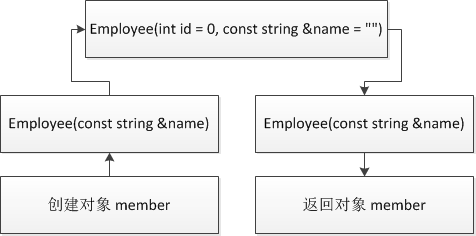
\includegraphics[width=0.5\textwidth]{FIG/exp6-2-1-4}
  \caption{创建~Employee~对象~member~的过程}
\end{figure}
\end{itemize}
\end{frame}
%--------------------
%#####################################
\subsection{复制构造函数}
\begin{frame}[fragile]
    {6.2.2 复制构造函数}

\begin{blueblock}<1->{示例}
复制一个已存在对象的内容来创建对象
\begin{lstlisting}
int i(1), j(i);
Fraction a(1, 5); //直接初始化
Fraction b(a);//直接初始化,b 为对象 a 的拷贝
\end{lstlisting}\vspace{-1.5mm}
\end{blueblock}


\begin{block}<2->{复制构造函数(copy constructor\index{C!constructor!copy constructor})}
\begin{itemize}
  \item 功能是将给定对象的数据成员依次复制给正在创建的对象;
  \item 复制构造函数的形参必须是\alert{引用类型},即给定实参的引用;
  \item 编译器会自动合成: 逐个成员\alert{按值复制},数组成员按元素逐个复制。
\end{itemize}
\end{block}
\begin{blueblock}<3->{定义形式}
 \vspace{-2.5mm}\begin{lstlisting}
class Fraction {
public:
    Fraction(const Fraction &rhs) : m_numerator(rhs.m_numerator),
        m_denominator(rhs.m_denominator) {  }
};
\end{lstlisting}\vspace{-1.5mm}
\end{blueblock}
\end{frame}

%--------------------
\begin{frame}[fragile]
    {6.2.2 复制构造函数}
\begin{columns}
\column{0.55\textwidth}
\begin{greenblock}{问题:下面代码是否正确?}
 \vspace{-2.5mm}\begin{lstlisting}
class Fraction {
public:
    Fraction(Fraction rhs):
        m_numerator(rhs.m_numerator),m_denominator(rhs.m_denominator) {}
};
int main(){
    Fraction a;
    Fraction b(a);
}
\end{lstlisting}\vspace{-1.5mm}
\end{greenblock}
\column{0.45\textwidth}

\begin{itemize}
  \item<2->[]

\begin{figure}
  \centering
  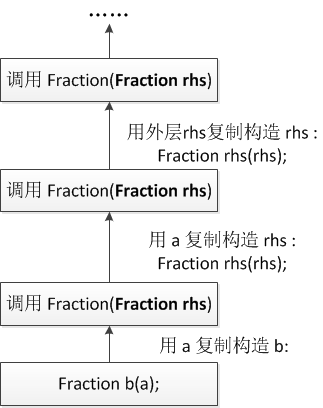
\includegraphics[width=0.8\textwidth]{FIG/exp6-2-2}
  \caption{无穷调用}
\end{figure}
\end{itemize}
\end{columns}
\end{frame}



%--------------------
\begin{frame}[fragile]
    {6.2.2 复制构造函数\small{~---~复制初始化}}
\begin{blueblock}{复制初始化例子}
 \vspace{-2.5mm}\begin{lstlisting}
Fraction c = Fraction(3, 2);
Fraction d = 7;
\end{lstlisting}\vspace{-1.5mm}
\end{blueblock}
\vspace{2em}
\begin{columns}
\column{0.45\textwidth}
\begin{itemize}
  \item<2->[]
\begin{figure}
%\vspace{-2em}
  \centering
  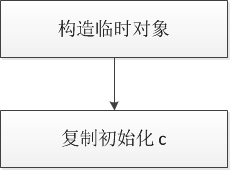
\includegraphics[width=0.6\textwidth]{FIG/exp6-2-2-1-b}
  \caption{Fraction c = Fraction(3, 2);}
\end{figure}
\end{itemize}
\column{0.45\textwidth}
\begin{itemize}
  \item<3->[]
\begin{figure}
\vspace{-2em}
  \centering
  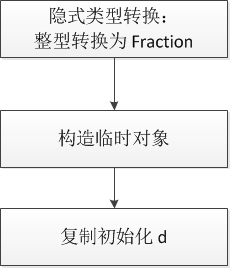
\includegraphics[width=0.6\textwidth]{FIG/exp6-2-2-1-a}
  \caption{Fraction d = 7;}
\end{figure}
\end{itemize}
\end{columns}
\end{frame}



\begin{frame}[fragile]
    {6.2.2 复制构造函数\small{~---~复制初始化}}

\begin{yellowblock}{直接初始化}
\begin{itemize}
  \item 使用普通函数匹配方式选择构造函数,没有临时对象的产生。
 \vspace{-1.5mm}\begin{lstlisting}
Fraction c(3, 2);
\end{lstlisting}\vspace{-1.5mm}
\end{itemize}
\end{yellowblock}

\begin{yellowblock}{复制初始化}
\begin{itemize}
  \item 将~=~右侧的对象复制给待创建对象;
  \item 类型不一致,编译器尝试通过构造函数进行类型转换;
  \item 如果没有可用构造函数,将产生类型无法转换的错误。
   \vspace{-1.5mm}\begin{lstlisting}
Fraction d = 7;
\end{lstlisting}\vspace{-1.5mm}
\end{itemize}

\end{yellowblock}

\end{frame}





\begin{frame}[fragile]
    {6.2.2 复制构造函数\small{~---~抑制隐式类型转换}}

\begin{block}{隐式类型转换的缺点}
\begin{itemize}
  \item 可能产生临时对象,带来程序性能的下降;
  \item 给用户带来意外,引起理解上的困难。。
\end{itemize}
\end{block}

\begin{block}{抑制隐式类型转换}
~\textcolor{blue}{explicit}\index{E!explicit}~关键字来阻止隐式类型转换,例子:\\
\begin{lstlisting}
class Fraction {
public:
    explicit Fraction(int above = 0, int below = 1) :
        m_numerator(above), m_denominator(below) {  }
};
\end{lstlisting}\vspace{-1.5mm}

\begin{itemize}
  \item<2->[]
  \vspace{-2.5mm} \begin{lstlisting}
Fraction d2 = 7; //错误:无法将 int 类型转换为 Fraction 类型
\end{lstlisting}\vspace{-1.5mm}
  \item<3->[]
 \vspace{-1.5mm}   \begin{lstlisting}
Fraction d2 = static_cast<Fraction>(7);//正确,强制类型转换
\end{lstlisting}\vspace{-1.5mm}
\end{itemize}


\end{block}

\end{frame}

%--------------------
\begin{frame}[fragile]
    {6.2.2 复制构造函数\small{~---~阻止复制}}

\begin{block}{复制构造函数的使用}
\begin{itemize}
  \item 将一个对象作为实参传递给一个非引用类型形参;
  \item 函数返回值类型为非引用类型对象;\label{chap6-2-2-return-by-value}
\end{itemize}
\end{block}


\end{frame}



%--------------------
\begin{frame}[fragile]
    {6.2.2 复制构造函数\small{~---~阻止复制}}
%\vspace{-3em}
\begin{columns}
\column{0.78\textwidth}
\begin{blueblock}{示例}
~divide~函数:用来实现两个分数的相除运算,返回结果为一个分数类型。
\begin{lstlisting}
Fraction divide(Fraction dividend, Fraction divisor) {
    Fraction result(divident.numerator()*divisor.denominator(),
         divident.denominator()*divisor.numerator());
    return result;
}

Fraction e = divide(b, c);
\end{lstlisting}\vspace{-1.5mm}
\onslide<2-> 调用几次构造函数?
\end{blueblock}
\column{0.2\textwidth}
\begin{figure}
%\vspace{-2em}
  \centering
  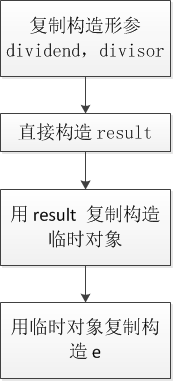
\includegraphics[width=1\textwidth]{FIG/exp6-2-2-3}
  \caption{~divide~函数}
\end{figure}
\end{columns}
\end{frame}



\begin{frame}[fragile]
    {6.2.2 复制构造函数\small{~---~阻止复制}}

\begin{greenblock}{阻止复制}

  \begin{lstlisting}
class Employee {
public:
    Employee(const Employee &) = delete;//阻止复制
};

Employee e1;  //调用默认构造函数
Employee e2(e1); //错误:复制构造函数是删除的,不能调用
\end{lstlisting}\vspace{-1.5mm}
\end{greenblock}

\end{frame}


\begin{frame}[fragile]
    {6.2.2 复制构造函数\small{~---~复制优化}}

\begin{greenblock}{以下代码会输出什么?}
\vspace{-2.5mm}\begin{lstlisting}
Fraction::Fraction(const Fraction &rhs) : m_numerator(rhs.m_numerator),
    m_denominator(rhs.m_denominator) {
    cout<< "Copy constructor called" << endl;
}
Fraction c2 = Fraction(3, 2);
\end{lstlisting}\vspace{-1.5mm}
\end{greenblock}
\begin{block}<2->{复制优化}
C++~编译器使用一种名为\alert{拷贝去除}(copy ellision\index{C!constructor!copy ellision})的优化技术:创建临时对象和调用拷贝构造函数这两个过程完全可以用直接初始化的方式来完成。
\end{block}

\begin{greenblock}<3->{使用引用提高代码性能}
\vspace{-1.5mm}
\begin{lstlisting}
Fraction divide(const Fraction &dividend, const Fraction &divisor) {
    return Fraction(divident.numerator()*divisor.denominator(),divident.denominator()*divisor.numerator());//返回值优化
}
Fraction b(2,3),c(4,5);
Fraction e = divide(b, c);
\end{lstlisting}\vspace{-1.5mm}
\onslide<4->divide函数调用过程中Fraction类构造函数调用几次?
\end{greenblock}

\end{frame}



\subsection{析构函数}
\begin{frame}[fragile]
    {6.2.3 析构函数}

\begin{block}{析构函数(destructor\index{D!destructor})}
\begin{itemize}
  \item 一个对象生命期结束时,编译器会自动调用;
  \item 销毁对象的所有成员;
  \item 名字由\alert{波浪号}紧接类名构成,不能有返回值,也不能包含形参。
\end{itemize}
\end{block}
\begin{blueblock}<2->{示例}
 \vspace{-2.5mm}\begin{lstlisting}
 class Fraction {
public:
    ~Fraction() { } //析构函数
};
\end{lstlisting}\vspace{-1.5mm}
\end{blueblock}

\begin{block}<3->{析构函数的行为}
\begin{itemize}
  \item 先执行函数体,然后按照初始化的顺序逆序销毁每个成员;
  \item 类类型的成员执行自己的析构函数;
  \item 释放对象成员在生命期内被分配的所有资源。
\end{itemize}
\end{block}

\end{frame}

\begin{frame}[fragile]
    {6.2.3 析构函数}
\begin{columns}
\column{0.65\textwidth}
\begin{block}{构造函数和析构函数的调用}
 \vspace{-2.5mm}\begin{lstlisting}
class Point {
    double m_x = 0, m_y = 0;
public:
    Point(double x=0,double y=0):m_x(x),m_y(y) {
        cout << "Constructor of Point" << endl;
    }
    Point(const Point &p) :m_x(p.m_x), m_y(p.m_y) {
        cout << "Copy constructor of Point" << endl;
    }
    ~Point() { cout << "Destructor of Point" << endl; }
};
class Circle {
    Point m_center;   double m_radius = 1.0;
public:
    Circle(double r = 1, const Point &p = Point()) :
        m_center(p), m_radius(r) {
        cout<<"Constructor of Circle"<<endl;
    }
    ~Circle() { cout<<"Destructor of Circle"<<endl;}
};
\end{lstlisting}\vspace{-1.5mm}
\end{block}
\column{0.33\textwidth}
\begin{block}{构造和析构}
 \vspace{-2.5mm}\begin{lstlisting}

{
    Circle a(2,Point(1,1));
}
Constructor of Point
Copy constructor of Point
Constructor of Circle
Destructor of Point
Destructor of Circle
Destructor of Point
\end{lstlisting}\vspace{-1.5mm}
\end{block}
\end{columns}
\end{frame}

\section{运算符重载}


\begin{frame}[fragile]
    {6.3 运算符重载}

\begin{blueblock}<1->{通过Fraction类辅助函数print打印一个对象~obj}
\vspace{-1.5mm}
\begin{lstlisting}
ostream& print(ostream &out, const Fraction &f) {
    out << f.m_numerator << "/" << f.m_denominator;
    return out;
}

Fraction obj ;
print(cout, obj);
\end{lstlisting}\vspace{-1.5mm}
\end{blueblock}

\begin{blueblock}<2->{通过运算符~\texttt{<<}~打印一个对象~obj}
\vspace{-1.5mm}
\begin{lstlisting}
Fraction obj ;
cout << obj ;
\end{lstlisting}\vspace{-1.5mm}
\end{blueblock}


\begin{block}<3->{运算符重载}
\begin{itemize}
  \item 将运算符作用于类类型对象,重新赋予新的含义;
  \item 增强代码的可读性。
\end{itemize}
\end{block}
\end{frame}

\subsection{基本概念}
\begin{frame}[fragile]
    {6.3.1 基本概念}
\begin{block}{运算符重载}
\begin{itemize}
  \item 由关键字~\textcolor{blue}{operator}\index{O!operator!operator overloading}~和需要重载的运算符共同组成;
  \item 重载的运算符的返回值类型以及参数列表由运算符的性质来决定:
  \begin{itemize}
    \item 一元运算符有一个参数;
    \item 二元运算符有两个参数,左侧运算对象传递给第一个参数,右侧运算对象传递给第二个参数
  \end{itemize}
\end{itemize}
\end{block}
\end{frame}

\begin{frame}[fragile]
    {6.3.1 基本概念}
\begin{blueblock}<1->{为~Fraction~类重载算术运算符~/,实现两个分数的除法运算}
\begin{itemize}
  \item<1->[]
 \vspace{-2.5mm}\begin{lstlisting}
 Fraction operator/(const Fraction &left, const Fraction &right) {
    Fraction result(left.numerator()*right.denominator(),
         left.denominator()*right.numerator());
    return result;
}
\end{lstlisting}\vspace{-1.5mm}
\end{itemize}
\end{blueblock}

\begin{columns}
\column{0.45\textwidth}
\begin{itemize}
  \item<2->[]
\begin{blueblock}{调用方式1:}
\begin{lstlisting}
Fraction a, b;
a \ b;
\end{lstlisting}\vspace{-1.5mm}
\end{blueblock}
\end{itemize}
\column{0.45\textwidth}
\begin{itemize}
  \item<3->[]
\begin{blueblock}{调用方式2:}
\begin{lstlisting}
Fraction a, b;
operator/(a, b);  //与 a / b 等价
\end{lstlisting}\vspace{-1.5mm}
\end{blueblock}
\end{itemize}
\end{columns}
\end{frame}

\begin{frame}[fragile]
    {6.3.1 基本概念}
\begin{block}{运算符函数作为类的成员函数:}
\begin{itemize}
  \item 成员运算符函数的显式参数比运算符的目数少一个;
  \item 运算符函数的第一个运算对象与隐含的~this~指针绑定。
\end{itemize}
\end{block}
\end{frame}

\begin{frame}[fragile]
    {6.3.1 基本概念}
\begin{blueblock}<1->{示例}
\begin{itemize}
  \item<1->[]
 \vspace{-2.5mm}\begin{lstlisting}
class Fraction {
public:
    Fraction& operator*=(const Fraction &rhs) {
        m_numerator *= rhs.m_numerator;
        m_denominator *= rhs.m_denominator;
        return *this;
    }
};
\end{lstlisting}\vspace{-1.5mm}
\end{itemize}
\end{blueblock}

\begin{columns}
\column{0.45\textwidth}
\begin{itemize}
  \item<2->[]
\begin{blueblock}{调用方式1:}
\begin{lstlisting}
Fraction a, b;
a *= b;
\end{lstlisting}\vspace{-1.5mm}
\end{blueblock}
\end{itemize}
\column{0.45\textwidth}
\begin{itemize}
  \item<3->[]
\begin{blueblock}{调用方式2:}
\begin{lstlisting}
Fraction a, b;
a.operator *= (b); //与 a *= b 等价
\end{lstlisting}\vspace{-1.5mm}
\end{blueblock}
\end{itemize}
\end{columns}

\begin{redblock}<4->{提示}
不可重载运算符:::、.、?:~和~.*。
\end{redblock}
\end{frame}


%#####################################
\subsection{重载原则}
\begin{frame}[fragile]
    {6.3.2 重载原则}
\begin{block}{1.~含义与内置类型一致}
 \vspace{-2.5mm}\begin{lstlisting}
 bool operator==(const Fraction &left, const Fraction &right) {
    return left.numerator()*right.denominator()==left.denominator()*right.numerator();
}
\end{lstlisting}\vspace{-1.5mm}
\end{block}
\begin{block}<2->{2.~行为与内置类型一致}
 \vspace{-2.5mm}\begin{lstlisting}
Fraction& Fraction::operator=(const Fraction &rhs) {//返回左值对象的引用
    if (&rhs == this) return *this;   //不会给自己赋值,例如, a = a;
    m_numerator = rhs.m_numerator;    m_denominator = rhs.m_denominator;
    return *this;
}
\end{lstlisting}\vspace{-1.5mm}
\end{block}

\begin{yellowblock}<3->{编译器会自动合成一个默认的赋值运算符}
\begin{itemize}
  \item 参数与返回值类型与上述函数一致;
  \item 将右侧对象的每个数据成员逐个赋值给左侧对象相应的数据成员;
  \item 对于数组成员,逐元素赋值。
\end{itemize}
\end{yellowblock}
\end{frame}

\begin{frame}[fragile]
    {6.3.2 运算符重载\small{~---~重载原则}}
\begin{block}{3.~成员函数的选择}
类成员函数还是类的辅助函数:
\begin{itemize}
  \item 赋值(=)、下标([])、函数调用(())和成员访问箭头(->)运算符必须是类成员;
  \item 改变运算对象自身状态的运算符应该是类成员,比如复合赋值、自增、自减运算符等;
  \item 具有对称性的运算符一般应作为类的辅助函数,比如算术、关系、逻辑运算符等。
\end{itemize}
\end{block}
\end{frame}

\begin{frame}[fragile]
    {6.3.2 重载原则}

\begin{yellowblock}<1->{提示}
\begin{itemize}
  \item<1-> 如果运算符作为类的成员函数,左侧对象一定是该类类型对象;
  \item<2-> 含有类类型的混合类型表达式,运算符应该定义成辅助函数,通常定义为\alert{友元函数}。
\begin{lstlisting}
class Fraction {
    friend Fraction operator/(int left, const Fraction &right);
};

Fraction operator/ (int left, const Fraction &right) {
    return Fraction(left*right.m_denominator, right.m_numerator);
}

Fraction a(1,2);
Fraction b = 4 / a;
\end{lstlisting}\vspace{-1.5mm}
\end{itemize}
\end{yellowblock}
\end{frame}




\begin{frame}[fragile]
    {6.3.2 重载原则}


\begin{block}<1->{4.~其它原则}
\begin{itemize}
  \item 只能重载~C++~语言已经存在的运算符,不能更改或创造新的运算符;
  \item 重载运算符的运算对象至少有一个是类类型。
\end{itemize}
\end{block}
\begin{greenblock}<2->{下面代码是否正确?}
\begin{itemize}
  \item <2->[]
   \vspace{-2.5mm}\begin{lstlisting}
int operator-(int, int);
\end{lstlisting}\vspace{-1.5mm}
  \item <3->[] 错误,不能重新定义内置运算符。
\end{itemize}

\end{greenblock}
\end{frame}


%#####################################
\subsection{输入和输出运算符}
\begin{frame}[fragile]
    {6.3.3 输入和输出运算符}
\begin{block}{输入和输出运算符}

重载~IO~标准库运算符~\verb;<<;~和~\verb;>>;~ 来实现输出和输入操作
,为了与~IO~标准库兼容,IO~运算符被声明为\alert{友元}。

\end{block}

\begin{blueblock}<2->{示例}
\begin{lstlisting}
class Fraction {
    friend ostream& operator <<  (ostream &os, const Fraction &a);
    friend istream& operator >>  (istream &is, Fraction &a);
};
\end{lstlisting}\vspace{-1.5mm}
\end{blueblock}
\end{frame}


\begin{frame}[fragile]
    {6.3.3 输入和输出运算符}
\begin{block}{重载输出运算符}
\begin{itemize}
  \item 第一个形参是一个非常量~ostream~类对象,需要向其写入数据;
  \item 第二个形参是类的常量引用,避免对实参进行写操作;
  \item 返回~ostream~类对象的引用。
\end{itemize}
\end{block}

\begin{block}<2->{示例}
 \vspace{-2.5mm}\begin{lstlisting}
ostream& operator <<  (ostream &os, const Fraction &a) {
    os << a.m_numerator << a.m_denominator;
    return os;
}
\end{lstlisting}\vspace{-1.5mm}
\end{block}

\begin{yellowblock}<3->{必须返回~ostream~类对象的引用}

\onslide<4-> 与运算符\texttt{<<}行为一致(连续输出);不允许复制IO类对象
\begin{lstlisting}
Fraction a, b;
cout << a << b << endl;
\end{lstlisting}\vspace{-1.5mm}

\end{yellowblock}

\end{frame}




\begin{frame}[fragile]
    {6.3.3 输入和输出运算符}
\begin{block}{重载输出运算符}
\begin{itemize}
  \item 第一个形参为~istream~类对象的引用,能返回~istream~类对象的引用;
  \item 第二个形参是类对象的常量引用,要对类对象进行写操作;
  \item 返回~istream~类对象的引用。
\end{itemize}
\end{block}

\begin{block}<2->{示例}
 \vspace{-2.5mm}\begin{lstlisting}
istream& operator >>  (istream &is, Fraction &a) {
    is >> a.m_numerator >> a.m_denominator;
    return is;
}

 Fraction a;
 cin >> a;
\end{lstlisting}\vspace{-1.5mm}
\end{block}

\end{frame}

\begin{frame}[fragile]
    {6.3.3 输入和输出运算符}
    \begin{itemize}
      \item 输入/输出运算符必须为类的辅助函数,不能作为类的成员函数,例如
    \end{itemize}
\begin{greenblock}<1->{下面程序是否有问题? }
\begin{lstlisting}
class Fraction {
public:
    istream& operator>>  (istream &is) {
        is >> m_numerator >> m_denominator;
        return is;
    }
};
int main() {
    Fraction a;
    cin >> a;
    return 0;
}
\end{lstlisting}\vspace{-1.5mm}
\end{greenblock}
\end{frame}


\begin{frame}[fragile]
    {6.3.3 输入和输出运算符}
\begin{greenblock}<1->{答案}
\begin{lstlisting}
class Fraction {
public:
    istream& operator>>  (istream &is) {
        is >> m_numerator >> m_denominator;
        return is;
    }
};
int main() {
    Fraction a;
    a.operator>>(cin);//类的成员函数的调用方式
    return 0;
}


\end{lstlisting}\vspace{-1.5mm}
\end{greenblock}

\end{frame}
%#####################################
\subsection{递增和递减运算符}
\begin{frame}[fragile]
    {6.3.4 递增和递减运算符}
\begin{blueblock}{递增运算符的声明}
 \vspace{-2.5mm}\begin{lstlisting}
class Fraction {
public:
    Fraction operator++(); //前置版本
    Fraction operator++(int);//后置版本
};
\end{lstlisting}\vspace{-1.5mm}
\end{blueblock}

\begin{blueblock}<2->{前置递增}
 \vspace{-2.5mm}\begin{lstlisting}
Fraction& Fraction::operator++() {
    ++m_numerator;  //分子加1
    return *this;  //为了与内置版本行为一致,前置递增运算符返回对象的引用
}
\end{lstlisting}\vspace{-1.5mm}
\end{blueblock}

\begin{blueblock}<3->{后置递增}
 \vspace{-2.5mm}\begin{lstlisting}
Fraction Fraction::operator++(int) { //形参仅为区别于前置版本
    Fraction a(*this);  //保存当前值
    m_numerator++; //分子加1
    return a; //以值返回方式返回局部对象
}
\end{lstlisting}\vspace{-1.5mm}
\end{blueblock}
\end{frame}

%#####################################
 \subsection{函数调用运算符}\label{chap6-3-5}
\begin{frame}[fragile]
    {6.3.5 函数调用运算符}
\begin{block}{函数调用运算符}
一个类重载了函数调用运算符,可以通过函数的方式来使用该类的对象,该类的对象称为\alert{函数对象}(function object\index{F!function object})。
\end{block}
\begin{blueblock}<2->{示例}
在~Fraction~类里面重载函数调用运算符,该运算符函数有两个形参,分别用来设置分子和分母,返回调用对象的~const~引用
\begin{lstlisting}
class Fraction {
public:
    const Fraction& operator()(int a, int b) {
        m_numerator = a;
        m_denominator = b;
        return *this;
    }
};

Fraction f;
f(3, 5);  //调用函数调用运算符
\end{lstlisting}\vspace{-1.5mm}
\end{blueblock}

\end{frame}

\begin{frame}[fragile]
    {6.3.5 函数调用运算符}

\begin{yellowblock}<1->{函数调用运算符和普通函数}
和普通函数相比,函数对象不但能以函数方式使用,它还能存储状态,因此它比普通函数更加灵活。
\end{yellowblock}


\begin{redblock}<2->{提示:函数调用运算符可以重载}
一个类可以重载多个版本的函数调用运算符,但它们必须为类的非静态成员函数。
\end{redblock}

\end{frame}

%#####################################
 \subsection{类型转换运算符}\label{chap6-3-6}
\begin{frame}[fragile]
    {6.3.5 类型转换运算符}
\begin{block}{类型转换运算符(conversion operator\index{C!conversion operator})}
\begin{itemize}
  \item 将类类型数据转换成其它类型数据;
  \item 语法格式如下:\\
 \indent operator type () const;\\
\end{itemize}
\end{block}

\begin{blueblock}<2->{示例}
为~Fraction~类添加一个转换为~double~类型的类型转换运算符:
\begin{lstlisting}
class Fraction {
public:
    Fraction(int above = 0, int below = 1) :
        m_numerator(above), m_denominator(below) {}
    operator double() const {
        return 1.*m_numerator/m_denominator;
    }
};
\end{lstlisting}\vspace{-1.5mm}
\end{blueblock}

\end{frame}



\begin{frame}[fragile]
    {6.3.5 类型转换运算符}

\begin{greenblock}{问题:下面代码是否正确,为什么?}

\begin{itemize}
  \item<1->[]
\begin{lstlisting}
Fraction f = 2;
\end{lstlisting}\vspace{-1.5mm}
  \item<2->[]正确,将  \textcolor{blue}{int} 类型隐式转换成 Fraction 类型,然后进行构造。
  \item<3->[]
  \begin{lstlisting}
double x = 1.5 + f;
\end{lstlisting}\vspace{-1.5mm}
  \item<4->[] 正确,调用类型转换运算符,将 f 隐式转换成  \textcolor{blue}{double} 类型。
  \item<5->[]
  \begin{lstlisting}
int i = f;
\end{lstlisting}\vspace{-1.5mm}
 \item<6->[] 正确:首先将 f 隐式转换成  \textcolor{blue}{double} 类型,然后将   \textcolor{blue}{double} 类型 转换为  \textcolor{blue}{int} 类型。
\end{itemize}

\end{greenblock}

\end{frame}

\begin{frame}[fragile]
    {6.3.5 类型转换运算符}


\begin{block}<1->{类型转换运算符的特点}
\begin{itemize}
  \item 以隐式的方式调用;
  \item 没有显式的返回值类型,也没有形参;
  \item 必须为类的成员函数;
  \item 一般将类型转换运算符声明为~ \textcolor{blue}{const}~成员。
\end{itemize}
\end{block}
\begin{redblock}<2->{提示}
不要过度依赖类型转换运算符。
\end{redblock}
\end{frame}




 \section{静态成员}

 \begin{frame}[fragile]
    {6.4 静态成员}

\begin{block}{静态成员}
类的某些属性值并非属于每个对象,类对象共享,比如,兼职人员的小时工资。
\begin{itemize}
  \item 类对象共享;
  \item 与类相关联;
  \item 存储于一个公用的内存中。
\end{itemize}
\end{block}

\end{frame}

\subsection{声明静态成员}
\begin{frame}[fragile]
    {6.4.1 声明静态成员}

\begin{blueblock}<1->{示例:声明静态成员}
利用关键字~ \textcolor{blue}{static}~为~Fraction~类添加一个静态成员
\begin{lstlisting}
class PartTimeWorker {
    string m_name; //员工姓名
    double m_hours;//工作小时数
    static double ms_payRate;//小时工资
public:
    double salary();
    static double rate() {
        return ms_payRate;
    }
    static void initRate(double rate);
};
\end{lstlisting}\vspace{-1.5mm}
\end{blueblock}

\begin{block}<2->{说明}
\begin{itemize}
  \item 在成员声明之前加上关键字~ \textcolor{blue}{static}~使其与类相关联;
  \item 静态数据成员在程序启动时创建,在程序结束时消亡;
  \item 类型可以为常量、引用、指针、类类型。
\end{itemize}
\end{block}

\end{frame}

\begin{frame}[fragile]
    {6.4.1 声明静态成员}
\begin{yellowblock}{静态数据和类对象}
一个类的静态数据成员不属于类对象,类对象不包含任何静态数据成员。
\end{yellowblock}
\begin{greenblock}<2->{在静态成员函数内部能不能直接使用~this~指针?}
\begin{itemize}
  \item<3->[]不能,静态成员函数不与任何对象绑定,因此不包含~this~指针,也就是说不能直接访问普通成员,而且也不能声明为常量成员函数。
\end{itemize}
\end{greenblock}
\end{frame}


\subsection{使用静态成员}\label{chap6-4-2}

\begin{frame}[fragile]
    {6.4.2 使用静态成员}
\begin{block}{定义静态成员}
为静态数据成员不属于类对象,因此他们并不是由构造函数来初始化。它们必须放到\alert{类的外部定义和初始化}。
\begin{itemize}
  \item 在类外定义的时候必须要指明所属的类;
  \item 不能重复~\textcolor{blue}{static}~关键字。
\end{itemize}
\end{block}
\end{frame}



\begin{frame}[fragile]
    {6.4.2 使用静态成员}

\begin{blueblock}<1->{定义静态成员:在类外部提供初始值} \vspace{-2.5mm}
\begin{lstlisting}
class PartTimeWorker {//其他成员省略
    static double ms_payRate;//小时工资
};
double PartTimeWorker::ms_payRate = 7.53;
\end{lstlisting}\vspace{-1.5mm}
\end{blueblock}

\begin{blueblock}<2->{定义静态成员:在类内部提供初始值} \vspace{-2.5mm}
\begin{lstlisting}
class PartTimeWorker {//其它成员与前面一致
    static const int ms_maxHourWeek = 20;  //每周最长工作时间
};
const int PartTimeWorker::ms_maxHourWeek;//在类内部已经有了初始值,则在类外部不可以再提供初始值
\end{lstlisting}\vspace{-1.5mm}
\end{blueblock}

\begin{blueblock}<3->{定义静态成员:可以在类内部也可以在类外部定义静态成员函数}
静态成员函数~initRate~在类外的定义:
\begin{lstlisting}
void PartTimeWorker::initRate(double rate) {
    ms_payRate = rate;
}
\end{lstlisting}\vspace{-1.5mm}
\end{blueblock}
\end{frame}

\begin{frame}[fragile]
    {6.4.2 静态成员\small{~---~使用静态成员}}

\begin{blueblock}<1->{使用静态成员:在类外可以通过类名直接访问公有的静态成员} \vspace{-2.5mm}
\begin{lstlisting}
cout << PartTimeWorker::rate() << endl; //通过类名访问静态成员
\end{lstlisting}\vspace{-1.5mm}
\end{blueblock}

\begin{blueblock}<2->{使用静态成员:通过类对象来访问静态成员} \vspace{-2.5mm}
\begin{lstlisting}
PartTimeWorker w;
cout << w.rate() << endl;  //通过类对象访问静态成员函数
\end{lstlisting}\vspace{-1.5mm}
\end{blueblock}

\begin{blueblock}<3->{使用静态成员:成员函数内部可以直接访问静态成员}\vspace{-2.5mm}
\begin{lstlisting}
double PartTimeWorker::salary() {
    return ms_payRate * m_hours;  //类内使用静态数据成员
}
\end{lstlisting}\vspace{-1.5mm}
\end{blueblock}
\end{frame}





%#####################################


\section{类成员指针*}

 \begin{frame}[fragile]
    {6.5 类成员指针*}

\begin{block}{类成员指针(pointer to member\index{P!pointer!pointer-to-member})}
指向类的非静态成员的指针。
\end{block}

\end{frame}

\subsection{数据成员指针*}



\begin{frame}[fragile]
    {6.5.1 数据成员指针*}
\begin{block}{数据成员指针}
\begin{itemize}
  \item 需要指明类成员的类型;
  \item 需要显式指明成员所属的类。
\end{itemize}
\end{block}

\begin{blueblock}<2->{示例:类成员指针的定义}
定义一个指向~PartTimeWorker~类数据成员~m\_name 的指针:
\begin{lstlisting}
string  PartTimeWorker::*p1 = &PartTimeWorker::m_name;
auto p2 = &PartTimeWorker::m_name;//利用 auto 简化指针的定义
\end{lstlisting}\vspace{-1.5mm}
\end{blueblock}


\begin{blueblock}<3->{示例:类成员指针的使用}
数据成员指针没有和类对象关联,可以将指针成员作用于类的对象来访问类的成员。
\begin{lstlisting}
PartTimeWorker w1, *w2 = &w1;
cout << w1.m_name << endl;  //普通访问方式
cout << w1.*p1 << endl; //数据成员指针访问方式,等价于 w1.m_name
cout << w2->*p1 << endl; //数据成员指针访问方式,等价于 w2->m_name
\end{lstlisting}\vspace{-1.5mm}
\end{blueblock}
\end{frame}




\begin{frame}[fragile]
    {6.5.1 数据成员指针*}
\begin{redblock}{注意}
类的\alert{访问控制规则}同样适用于成员指针:\\
m\_name~为~PartTimeWorker~类的私有数据成员,因此上面的代码必须位于类的成员函数或类的友元函数中;否则,会出现编译错误。
\end{redblock}

\end{frame}





\subsection{成员函数指针}



\begin{frame}[fragile]
    {6.5.2 成员函数指针*}
\begin{block}{成员函数指针}
\begin{itemize}
  \item 需要指明类成员函数的类型;
  \item 需要显式指明成员函数所属的类。
\end{itemize}
\end{block}

\begin{blueblock}<2->{示例:成员函数指针的定义}
定义一个指向~PartTimeWorker~类的成员函数指针~pf,pf~可以指向~PartTimeWorker~类中返回类型为~double~且无参的成员函数。
\begin{itemize}
  \item<3->[]
  \begin{lstlisting}
double (PartTimeWorker::*pf)();
pf = &PartTimeWorker::salary;
\end{lstlisting}\vspace{-1.5mm}
  \item<4->[]
    \begin{lstlisting}
auto pf2 =  &PartTimeWorker::salary;
\end{lstlisting}\vspace{-1.5mm}
  \item<5->[]
  \begin{lstlisting}
using PTWS = double (PartTimeWorker::*)();
PTWS pf3 = &PartTimeWorker::salary;
\end{lstlisting}\vspace{-1.5mm}
\end{itemize}
\end{blueblock}


\end{frame}




\begin{frame}[fragile]
    {6.5.2 成员函数指针*}

\begin{blueblock}<1->{示例:类成员指针的使用}
需要使用~.*~或者~->*~运算符作用于指向成员函数的指针,来调用类成员函数。
\begin{lstlisting}
PartTimeWorker w;
cout << w.salary() << endl;  //普通调用方式
cout << (w.*pf)() << endl; //成员函数指针调用方式
\end{lstlisting}\vspace{-1.5mm}
\end{blueblock}

\begin{greenblock}<2->{(w.*pf)~的圆括号能否省略?}
\begin{itemize}
  \item<3-> (w.*pf)~的圆括号不能缺少,原因是函数调用运算符的优先级高于指向成员指针运算符的优先级。
\end{itemize}
\end{greenblock}


\end{frame}




\begin{frame}[fragile]
	\frametitle{~~}
	\begin{center}
		\huge{本章结束}
	\end{center}
\end{frame}

\end{document}
